%% 
%% Copyright 2019-2020 Elsevier Ltd
%% 
%% This file is part of the 'CAS Bundle'.
%% --------------------------------------
%% 
%% It may be distributed under the conditions of the LaTeX Project Public
%% License, either version 1.2 of this license or (at your option) any
%% later version.  The latest version of this license is in
%%    http://www.latex-project.org/lppl.txt
%% and version 1.2 or later is part of all distributions of LaTeX
%% version 1999/12/01 or later.
%% 
%% The list of all files belonging to the 'CAS Bundle' is
%% given in the file `manifest.txt'.
%% 
%% Template article for cas-dc documentclass for 
%% double column output.

%\documentclass[a4paper,fleqn,longmktitle]{cas-dc}
\documentclass[a4paper,fleqn]{cas-dc}

%\usepackage[authoryear,longnamesfirst]{natbib}
%\usepackage[authoryear]{natbib}
\usepackage[numbers]{natbib}

%%%Author definitions
\def\tsc#1{\csdef{#1}{\textsc{\lowercase{#1}}\xspace}}
\tsc{WGM}
\tsc{QE}
\tsc{EP}
\tsc{PMS}
\tsc{BEC}
\tsc{DE}
%%%
% -------------------------------------------------------------------
% Pacotes para inserção de figuras e subfiguras
\usepackage{subfig,epsfig,tikz,float}		            % Packages de figuras. 
\usepackage{graphicx}
\graphicspath{ {./figs/} }
% -------------------------------------------------------------------
% \usepackage{amssymb}
% -------------------------------------------------------------------
% Pacotes para inserção de tabelas
\usepackage{booktabs,multicol,multirow,tabularx,array}          % Packages para tabela
\usepackage{natbib}
\usepackage{pifont}
\usepackage{xcolor}
% -------------------------------------------------------------------
\PassOptionsToPackage{style=super,nolist}{glossaries}
\PassOptionsToPackage{acronym}{glossaries}
\PassOptionsToPackage{nonumberlist}{glossaries}
\usepackage{glossaries}
\newacronym{ai}{AI}{Artificial Intelligence}
\makeglossaries
% -------------------------------------------------------------------
\usepackage[utf8]{inputenc} % The default since 2018
\DeclareUnicodeCharacter{200B}{{\hskip 0pt}}
% -------------------------------------------------------------------
\begin{document}
\let\WriteBookmarks\relax
\def\floatpagepagefraction{1}
\def\textpagefraction{.001}
\shorttitle{Leveraging social media news}
\shortauthors{CV Radhakrishnan et~al.}


\title [mode = title]{Decentralized File Exchange Hub: A Cloud-Native Approach}                     

\credit{Conceptualization of this study, Methodology, Software}

\author[1]{Rafael Pereira}[type=editor,
                        %auid=000,bioid=1,
                        linkedin='rafaelmendespereira',
                        orcid=0000-0001-8313-7253]
%\cormark[1]
%\fnmark[1]
\ead{rafael.m.pereira@ipleiria.pt}
   
\address[1]{Computer Science and Communications Research Centre, School of Technology and Management, Polytechnic of Leiria, 2411-901 Leiria, Portugal}

\begin{abstract}

In this report, we present a decentralized file exchange hub designed using a cloud-native approach that leverages containers, microservices, and cloud services. Our architecture comprises a React-based frontend served by Nginx, an Express API for managing file transfers, a real-time communication server using Socket.IO, and MongoDB as the primary database. The application stores files in Google Cloud Storage, and our deployment pipeline is streamlined using Google Cloud Build and Cloud Run. The result is a scalable, resilient, and efficient file exchange system that demonstrates the power and flexibility of modern cloud computing technologies for software applications.

\end{abstract}

\begin{keywords}
Decentralized file exchange \sep Microservices architecture \sep Containerization \sep Cloud-native deployment \sep Real-time communication \sep Scalability and resilience
\end{keywords}


\maketitle

\section{Introduction}

The rapid growth of cloud computing and microservices has revolutionized the way applications are developed and deployed. As a result, there is an increasing need for effective strategies to manage the complexity and scalability of these systems. This report explores the design and deployment of a distributed cloud-based application that utilizes containerization and microservices to achieve high availability, performance, and maintainability.

The application is divided into four main modules: Presentation Provider (Nginx), API (Express), Asynchronous Message Communication server, and Database (MongoDB). Each module is designed to serve a specific purpose and can scale independently to adapt to changing loads and requirements. The application also leverages Google Cloud Platform (GCP) services such as Cloud Storage Bucket for storing and managing files.

The report is structured as follows: Section \ref{sec:architecture} presents the architecture of the application, detailing the purpose and design of each module. Section \ref{sec:deployment} describes the deployment process, emphasizing the use of GCP's Cloud Build and Cloud Run services to automate and streamline the deployment of the application components. Finally, the report concludes with a summary of the key findings and insights gained from the project.

\section{Architecture}\label{sec:architecture}

This project follows a microservices architecture, which allows for improved scalability, resilience, and maintainability. The system is divided into four main components, each responsible for a specific aspect of the application. Figure \ref{fig:architecture} presents a diagram of the architecture, illustrating the relationship between each component.

\begin{enumerate}
    \item Presentation Provider (Nginx): This component acts as the frontend server, hosting the React web application and serving static files. It is responsible for delivering the user interface to the clients and handling incoming HTTP requests.
    \item API (Express File Management Service): This component is the backend server implemented using Express.js. It manages the file uploading and downloading processes, interacting with the Database and Cloud Storage Bucket to store and retrieve files.
    \item Asynchronous Message Communication Server (Socket.io): This server enables real-time communication between the clients, ensuring that users in the same room receive instant updates when a new file is shared.
    \item Database (MongoDB): The database stores information about the rooms, users, and file metadata, including the bucket URL and timestamp. MongoDB was chosen for its flexibility, scalability, and performance.
    \item Cloud Storage Bucket (Azure Blob Storage): This component stores the uploaded files, providing a reliable and scalable storage solution.
\end{enumerate}

The following UML diagram (Figure \ref{fig:architecture}) depicts the relationships between the components:

\begin{figure}[h]
    \centering
    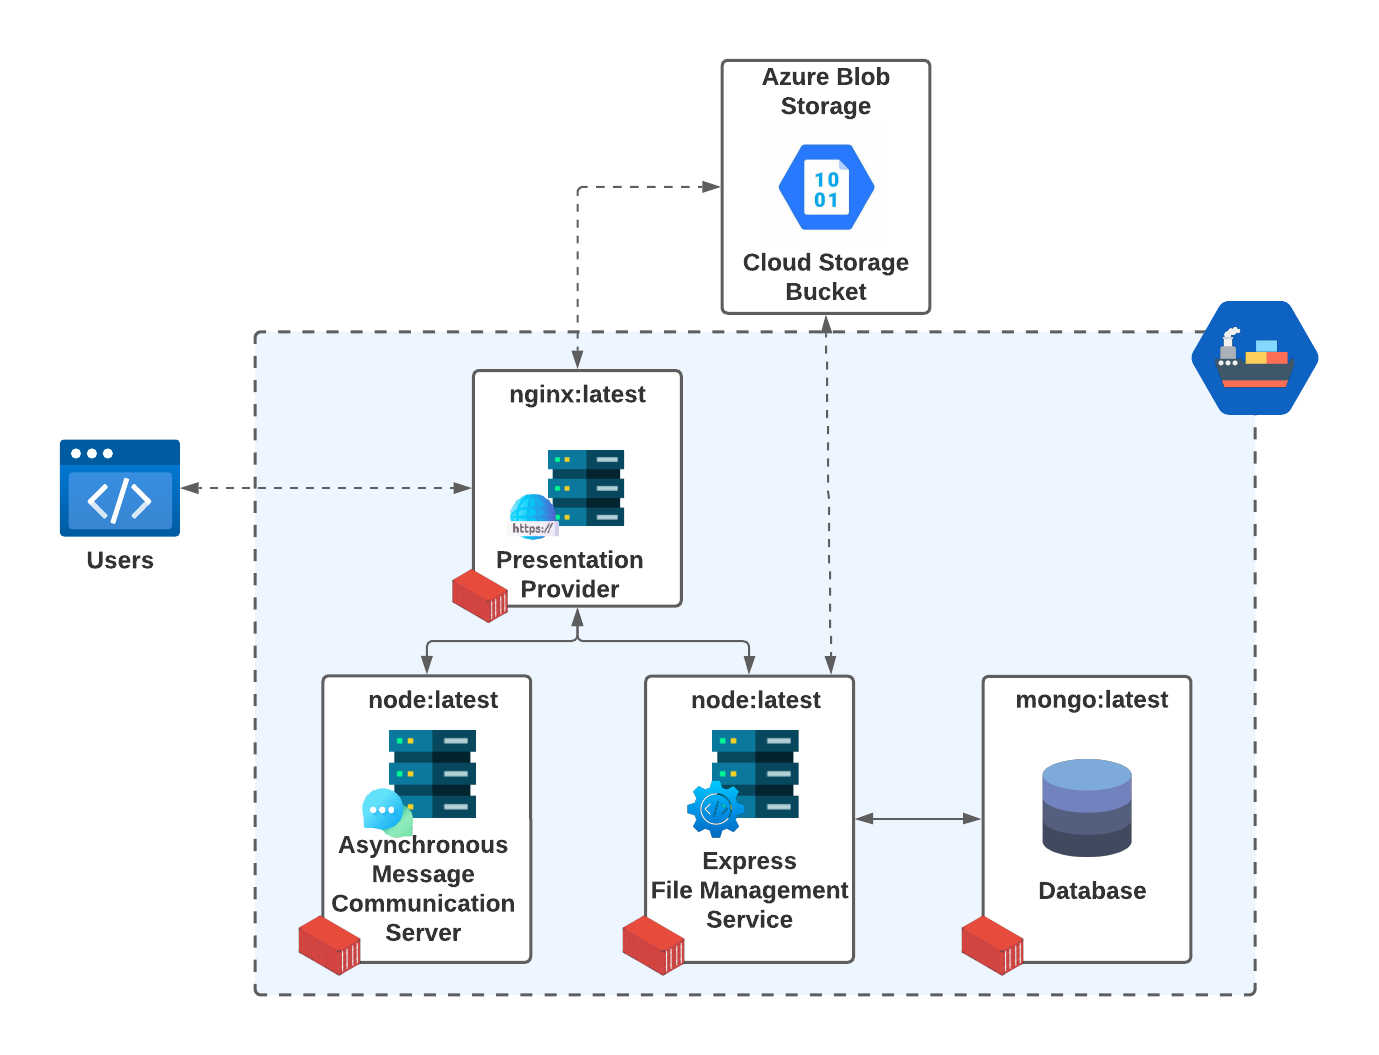
\includegraphics[width=9cm]{architecture.png}
    \caption{Local system architecture diagram.}
    \label{fig:architecture}
\end{figure}

In this architecture, each component communicates with the others through well-defined interfaces, allowing for efficient collaboration and easy maintenance. The use of containerization and cloud-native deployment further enhances the system's scalability and resilience.

\subsection{Presentation Provider: Nginx-based Frontend}

The presentation layer of our file exchange hub is built using a React web application. We utilize Nginx as a reverse proxy and web server to serve the static content generated by the React application. Nginx offers excellent performance, stability, and low resource usage, making it an ideal choice for our frontend. Furthermore, its ability to handle a large number of simultaneous connections ensures a responsive user experience, even during peak loads.

\subsection{API: Express-based File Transfer Service}

Our file transfer service is implemented using Node.js with the Express framework, providing a robust and scalable API for managing file uploads and downloads. This service is responsible for handling file metadata, coordinating file transfers, and integrating with the cloud storage service for actual file storage. Express is chosen for its ease of use, extensive documentation, and compatibility with Node.js, which allows for efficient development and seamless integration with other components.

\subsection{Asynchronous Message Communication Server: Socket.IO}

To enable real-time communication and notifications within our file exchange hub, we employ Socket.IO, a popular library for real-time web applications. This server facilitates instant messaging between users in the same room, ensuring a seamless and interactive experience for all participants. Socket.IO is selected for its flexibility, reliability, and compatibility with various platforms and transports, making it a powerful solution for real-time communication in our application.

\subsection{Database: MongoDB}

MongoDB, a NoSQL database, is utilized to store information about rooms, files, and users. It's flexible schema and horizontal scalability makes it a fitting choice for our cloud-native application, as it can easily adapt to changing requirements and handle large volumes of data. Additionally, MongoDB provides a rich query language and high-performance indexing capabilities, allowing for efficient data retrieval and manipulation.

\subsection{Cloud Storage Bucket: Azure Blob Storage}

To store and manage the actual files exchanged by users, we leverage Azure Blob Storage. This fully managed object storage service offers high availability, durability, and scalability, allowing our file exchange hub to efficiently store, retrieve, and share files. The choice of Azure Blob Storage is driven by its integration with other Azure services, its security features, and its cost-effective pricing model, making it a suitable solution for our application's file storage needs.

\section{Deployment} \label{sec:deployment}

The deployment process is designed to ensure a smooth transition from development to production, leveraging the power of Google Cloud Platform (GCP) services. The deployment strategy uses GCP's Cloud Build and Cloud Run services, along with GitHub Actions and Terraform, for automating and streamlining the process. Figure \ref{fig:deployment} presents a diagram of the deployment process, illustrating the steps and relationships between each involved service.

\begin{enumerate}
\item Cloud Build: This service automates the build and deployment of the application components. It is triggered by Terraform and pulls Docker images from Docker Hub, builds the application components, and pushes the images to Google Container Registry.
\item Cloud Run: This service deploys the containerized applications on a fully managed platform, providing automatic scaling and load balancing. It ensures that the services are highly available and resilient.
\end{enumerate}

The following diagram (Figure \ref{fig:deployment}) depicts the deployment process and the relationships between the components:

\begin{figure}[h]
\centering
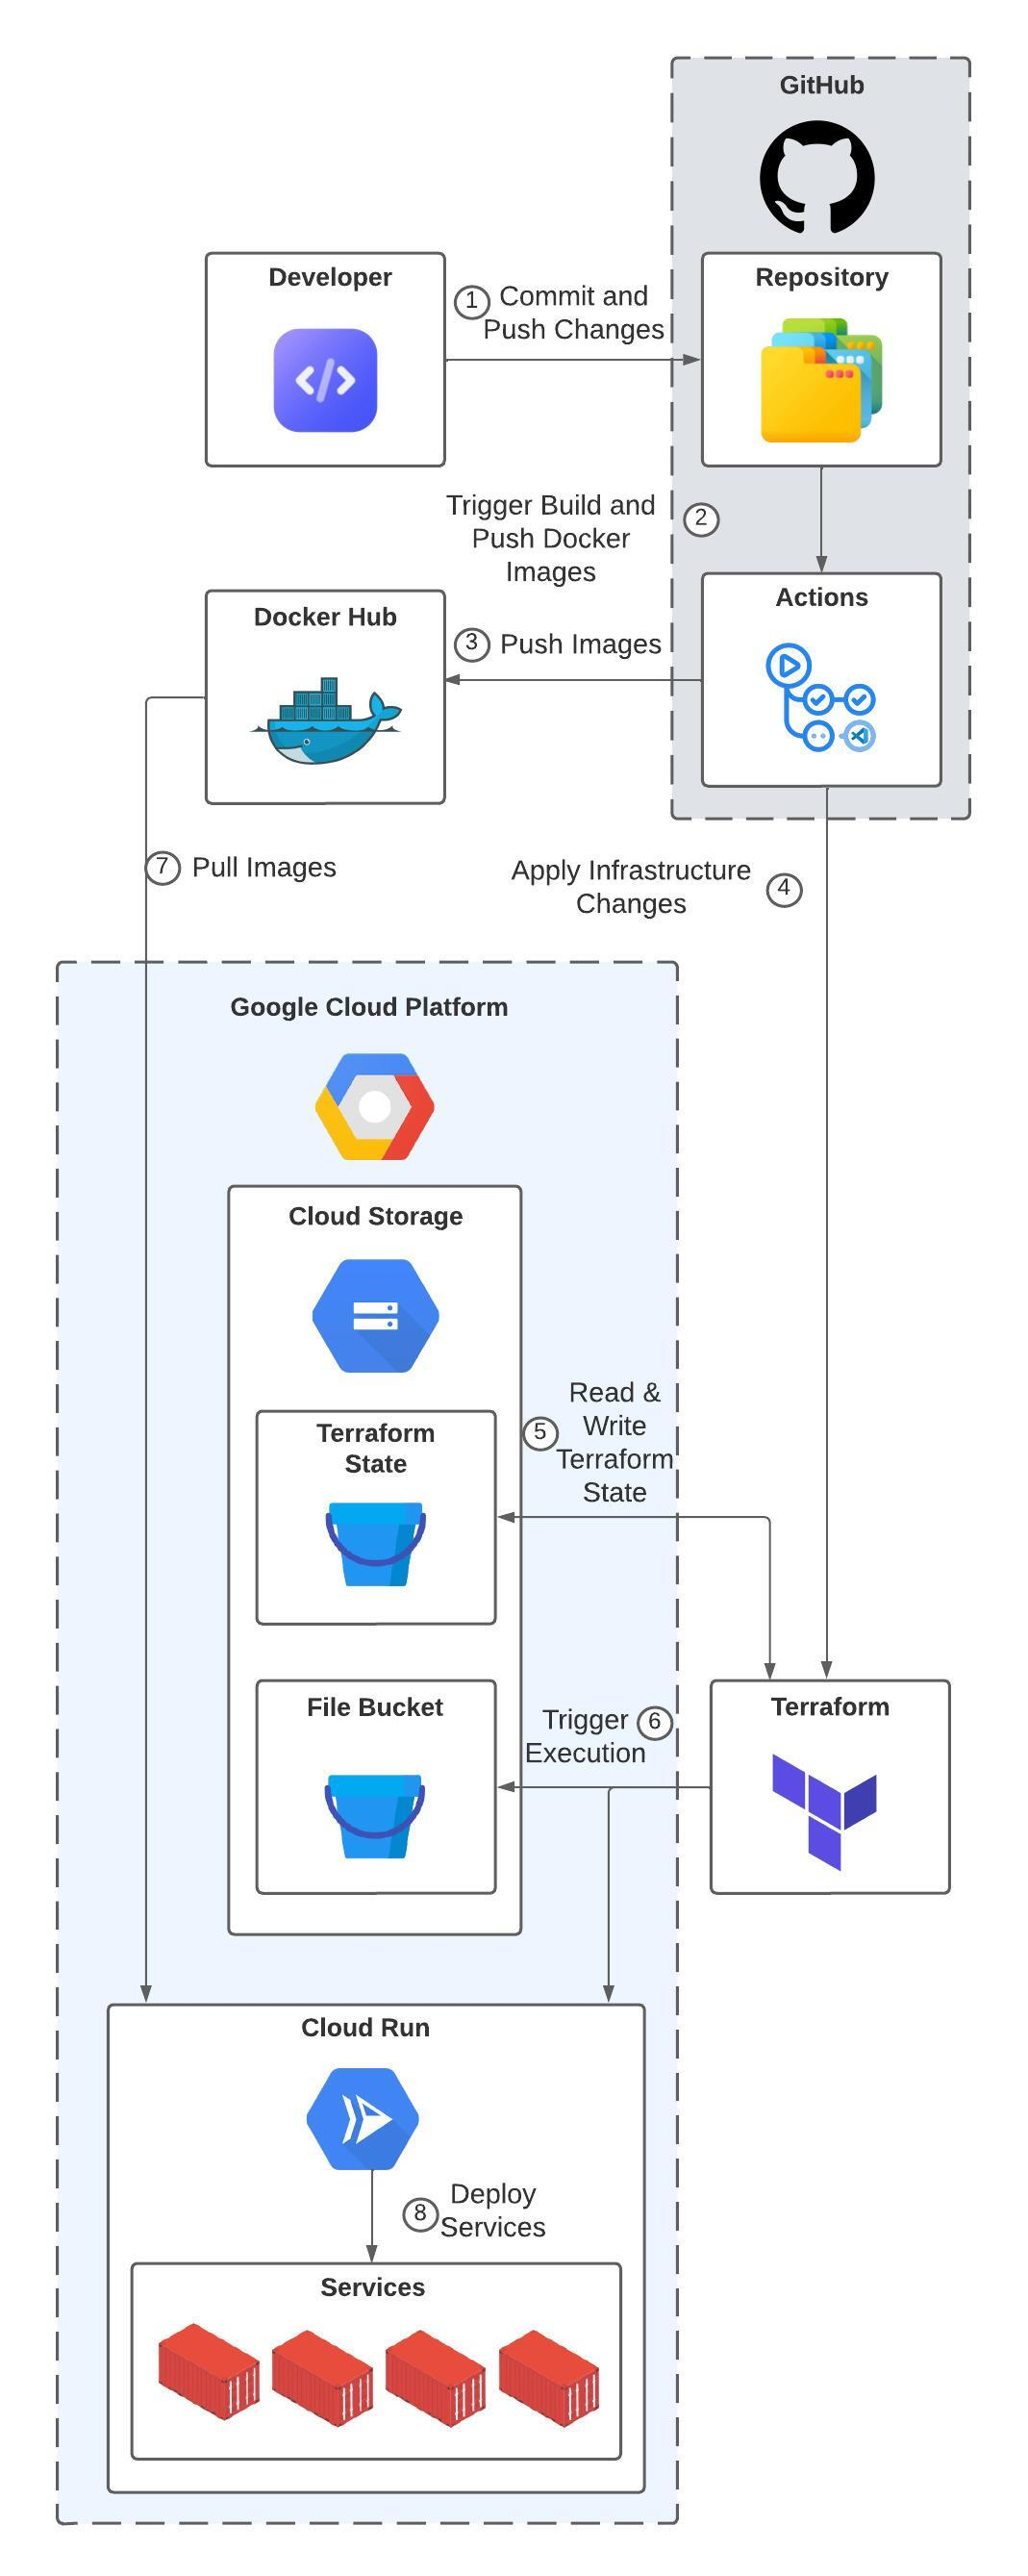
\includegraphics[width=8cm]{Deployment.jpeg}
\caption{Deployment process diagram illustrating the flow: (1) Developer commit and pushes changes to the repository, (2) triggering GitHub Actions to (3) build and push Docker images to Docker Hub. (4) Terraform is initiated, applying infrastructure changes and (5) triggering Cloud Build to (6) pull images from Docker Hub. Cloud Build builds the application components and (7) pushes the images to Google Container Registry. (8) Terraform triggers Cloud Run, which (9) pulls images from the Container Registry and (10) deploys the containerized services. (11) Cloud Run handles incoming requests from end user to the deployed services.}
\label{fig:deployment}
\end{figure}

The deployment process ensures that the application components are consistently built and deployed across environments, minimizing human error and facilitating continuous integration and delivery.

\subsection{Cloud Build: Continuous Integration and Deployment}

Google Cloud Build is a managed service that enables the automated building and deployment of applications in the Google Cloud Platform. It is triggered by Terraform and integrates with Docker Hub to pull the Docker images for the various services in the application. Once the images are pulled, Cloud Build builds the application components and pushes the images to Google Container Registry, making them ready for deployment on Google Cloud Run.

\subsection{Cloud Run: Scalable Containerized Services}

Google Cloud Run is a serverless platform that enables the deployment and management of containerized applications. By leveraging the power of containers, Cloud Run allows developers to focus on writing code without worrying about the underlying infrastructure. The platform automatically scales applications based on demand, ensuring optimal resource usage and minimizing costs.

\subsection{Automated Continuous Deployment with GitHub Actions and Terraform}

In order to streamline the deployment process and ensure a consistent and efficient release cycle, we implemented Continuous Deployment using GitHub Actions and Terraform. GitHub Actions automates the process of building and pushing Docker images to Docker Hub, while Terraform manages the infrastructure required to deploy and update the services on Google Cloud Run.

When changes are pushed to the repository, GitHub Actions triggers an automated workflow that builds and pushes the updated Docker images for each microservice to Docker Hub. Following the successful completion of this step, the workflow then initiates the Terraform CLI to manage the deployment of the microservices to Google Cloud Run.

Using Terraform, we define the infrastructure for each microservice as code, including Google Cloud Run services and IAM policies. This approach enables us to maintain a version-controlled and easily auditable infrastructure while also allowing for seamless updates and configuration changes. By integrating with GitHub Actions, we ensure that every push to the repository automatically triggers a new deployment, resulting in a streamlined and consistent release process.

\section{Conclusion}

This report has presented a decentralized file exchange hub designed with a cloud-native approach. By leveraging containers, microservices, and cloud services, we have created a scalable, resilient, and efficient system for exchanging files. Our use of modern technologies such as Nginx, Express, Socket.IO, MongoDB, and Google Cloud Platform services demonstrates the power and flexibility of cloud computing for modern software applications. Additionally, the integration of GitHub Actions, Google Cloud Build, Terraform, and Google Cloud Run has streamlined the deployment process, providing a robust Continuous Integration and Continuous Deployment (CI/CD) pipeline for ensuring consistent and reliable application delivery. The decentralized file exchange hub showcases the potential for creating high-performance, scalable, and flexible systems using cutting-edge cloud technologies and best practices.

%% Loading bibliography style file
%\bibliographystyle{model1-num-names}
%\bibliographystyle{cas-model2-names}
%\bibliographystyle{unsrt} % Estilo de Bibliografia
% Loading bibliography database
%\bibliography{cas-refs}


%\vskip3pt

\end{document}
